\subsection{Physcis of Proton-Proton Collisions}

\begin{figure}[htb]
  \begin{center}
    {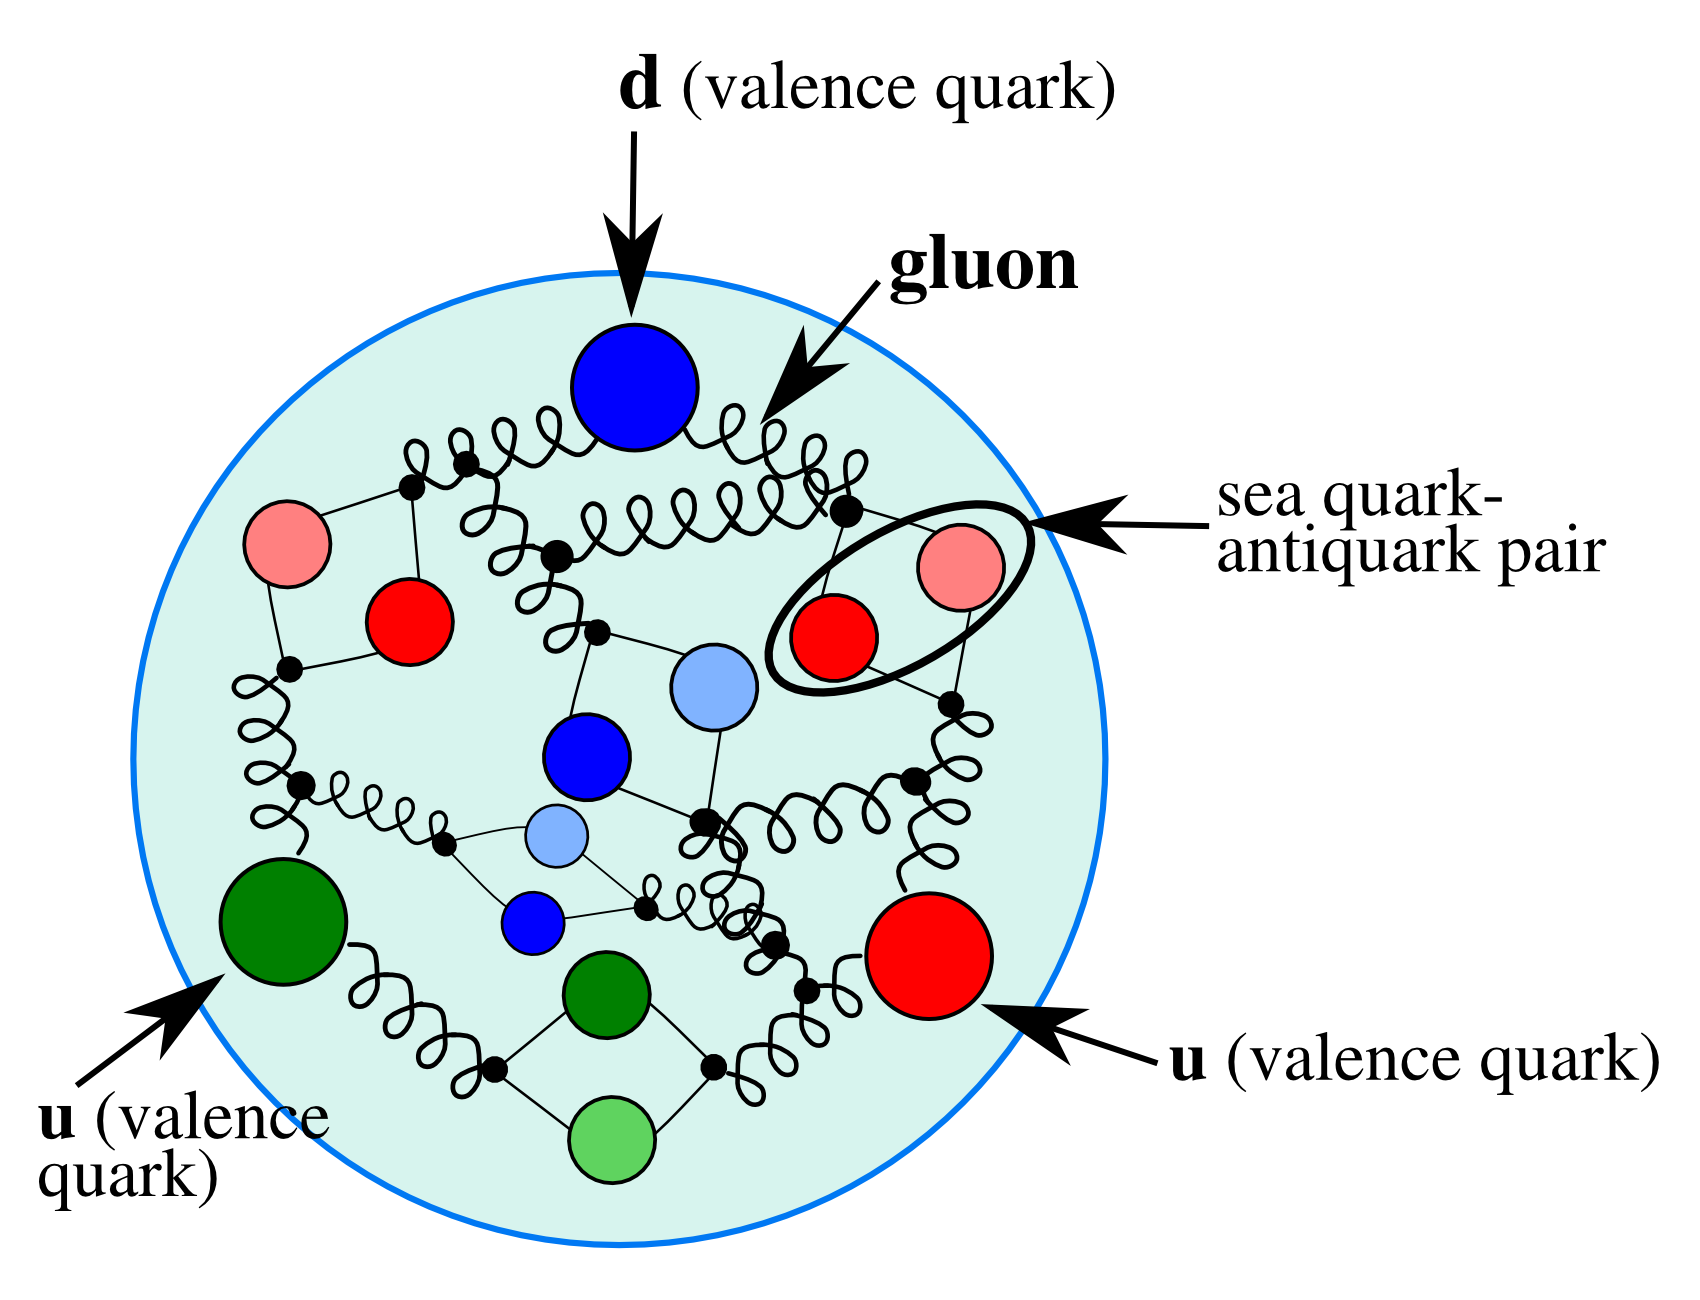
\includegraphics[width=0.45\textwidth]{../figs/Intro/protonStructure.png}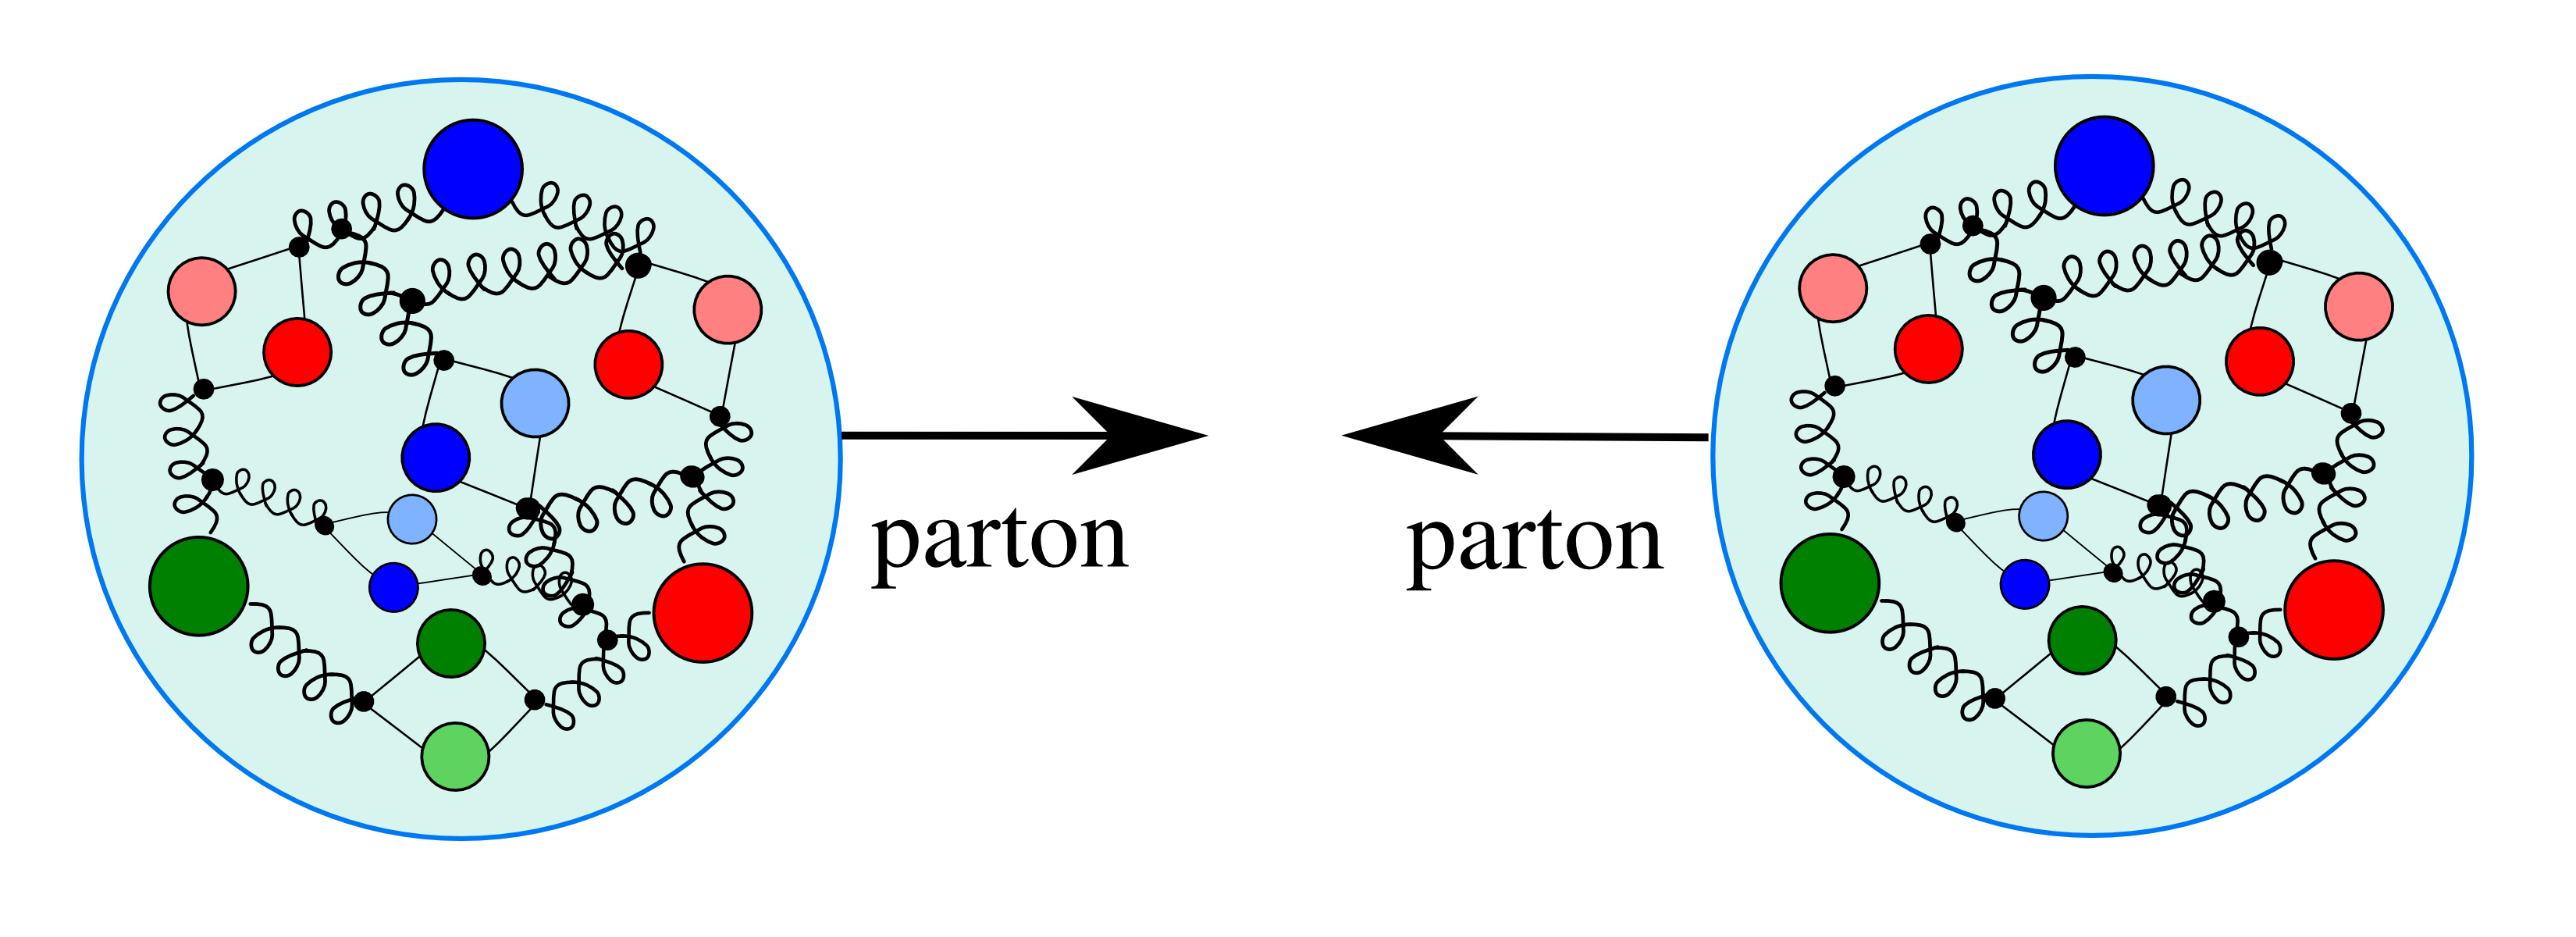
\includegraphics[width=0.45\textwidth]{../figs/Intro/ppCollision.png}}
    \caption{The proton structure (left) and the proton-proton collision (right).}
    \label{fig:ppCollision}
  \end{center}
\end{figure}

The schemes of the proton structure and a proton-proton collision are shown in Fig. \ref{fig:ppCollision}. A proton consists of three quarks: uud. An electric charge of a proton is a sum of the quarks charges: Q=+2/3+2/3-1/3=1. The situation with the mass is different: the mass of a u quark is 6 GeV and the mass of a d quark is 3 GeV while the mass of a proton is 940 GeV. The mass of a proton is an invariant mass of a system of the quarks which is mostly comprised of their kinetic energy. These three quarks are called valence quarks. They interact with each other by exchanging gluons. Gluons emit other gluons and produce $q\bar{q}$ pairs. Such virtual quarks are called sea quarks.

If two low energetic protons interact, it corresponds to the large distance between them and such protons do not probe one another's structure. They see each other as colorless electrically charged particles and therefore interact electromagnetically by exchanging a photon. Protons of higher energy see one another's intrinsic structure: its constituents, quarks, antiquarks and gluons, interact strongly with each other. Valence quarks, as well as sea quarks and antiquarks, can participate in the couplings.

In LHC collisions quark-(anti)quark, gluon-(anti)quark, gluon-gluon interactions are all possible however at such high energies, gluon-gluon interactions are prevalent. That is why the LHC sometimes is being called the gluon collider.

One important specific of high energetic proton collisions is the fact that an interacting particle possesses only part of a proton energy and momentum. Therefore, the energies and longitudinal momenta of the initial state particles are unknown. Although, the total transverse momenta is known to be equal to zero.  
